\chapter{Weakly Acyclic Languages}\label{chapter:weakly_acyclic_language}

In this chapter we introduce a class of formal languages, which we call weakly acyclic. They are a subset of the regular languages and are characterized by having no cycles beyond self-loops in the automata representation.

\section{Weakly Acyclic DFAs}\label{sec:weakly_acyclic_dfa}

\begin{definition}[\cite{blondin_24}]
Let $A = (Q, \Sigma, q_{0},\delta,F)$ be a DFA and let $\alpha(w)$ be the set of letter, which occur within in word $w$. DFA $A$ is weakly acyclic, if $\delta(q,w) = q$ implies $\delta(q,a) = q$ for every $a \in \alpha(w)$
\end{definition}

The following definitions are equivalently expressing, that a DFA $(Q, \Sigma, q_{0},\delta,F)$ is \textit{weakly acyclic}:
\begin{itemize}[--,noitemsep]
	\item the binary relation $\precsim $  over $Q \times Q$ with $q \precsim q'$ if $\delta(q,w) = q'$ is a partial order
	\item each strongly connected component of underlying directed graph contains a single state 
	\item the underlying directed graph does not contain any simple cycle except from self-loops
\end{itemize}

\autoref{fig:wadfa} shows an example for a weakly acyclic DFA and \autoref{fig:notwa} illustrates two not weakly acyclic DFAs.

\begin{figure}[H]
\begin{tikzpicture}[shorten >=1pt,node distance=2.5cm,on grid,>={Stealth[round]},auto]

  \node[state,initial]  (q1)                      {$q_1$};
  \node[state]          (q2) [above right=of q1] {$q_2$};
  \node[state]          (q3) [right=of q1] {$q_3$};
  \node[state]			(q4) [right=of q2] {$q_4$};
  \node[state,accepting](q5) [right=of q3] {$q_5$};
  \node[state](q6) [right=of q4] {$q_6$};
  
  \draw   (q1) edge[above] node{$\bm{b}$} (q2)
          (q1) edge[above] node{$\bm{a}$} (q3)
          (q3) edge[loop above] node{$\bm{a}$} (q2)
          (q3) edge[above] node{$\bm{b}$} (q5)
%          (q2) edge[above] node{$\bm{b}$} (q5)
          (q2) edge[above] node{$\bm{a},\bm{b}$} (q4)
          (q4) edge[right] node{$\bm{b}$} (q5)
          (q5) edge[loop right] node{$\bm{a},\bm{b}$} (q5)
          (q4) edge[above] node{$\bm{a}$} (q6)
          (q6) edge[loop right] node{$\bm{a},\bm{b}$} (q6);  
\end{tikzpicture}
%\begin{tikzpicture}[shorten >=1pt,node distance=2.1cm,on grid,>={Stealth[round]},auto]
%
%  \node[state,initial]  (q_0)                      {$q_1$};
%  \node[state]          (q_1) [above right=of q_0] {$q_2$};
%  \node[state]          (q_2) [below right=of q_0] {$q_3$};
%  \node[state,accepting](q_3) [below right=of q_1] {$q_4$};
%
%  \path[->] (q_0) edge               node         {$\bm{a}$} (q_1)
%                  edge               node [swap] {$\bm{b}$} (q_2)
%            (q_1) edge               node         {$\bm{a}$} (q_3)
%                  edge [loop above] node         {$\bm{b}$} ()
%            (q_2) edge               node [swap] {$\bm{b}$} (q_3)
%                  edge [loop below] node         {$\bm{a}$} ()  
%            (q_3) edge [loop right]  node  {$\bm{a},\bm{b}$} ();
%                  
%\end{tikzpicture}
    	\caption{Example of a Weakly Acyclic DFA}\label{fig:wadfa}
\end{figure}

\begin{lemma}\label{lem:minimal}
Let $A$ be a weakly acyclic DFA. The minimal DFA that accepts L$(A)$ is also weakly acyclic. 
\end{lemma}

\begin{proof}
See {\cite[Proposition~4]{blondin_24}}
\end{proof}



\section{Other Representations}

As with regular languages, there are equivalent ways to represent weakly acyclic languages. Let $\alpha(w)$ be the set of letter, which occur within in word $w$. 
Blondin et al. have shown that weakly acyclic DFAs, weakly acyclic NFAs and weakly acyclic expressions represent the same class of weakly acyclic languages \cite{blondin_24}. 


%It can further be shown, that if a weakly acyclic DFA $A$ accepts the language $L(A)$, then the minimal automata for this language is also weakly acyclic \cite{blondin_24}. 

\subsection{Weakly Acyclic NFAs}
An NFA $(Q, \Sigma, q_{0},\delta,F)$ is \textit{weakly acyclic} if 
\begin{itemize}[--,noitemsep]
	\item $q \in \delta(q,w)$ implies $\delta(q,a) = {q}$ for every $a \in \alpha(w)$
	\item the underlying directed graph does not contain any simple cycle except from self-loops and non-determinism with a letter $a$ can only appear from a state with no self-loop of $a$.
\end{itemize}

\subsection{Weakly Acyclic Expressions}\label{sec:weakly_acyclic_regex}
The class of weakly acyclic languages can also be characterized by \textit{weakly acyclic expressions} of the following form:
\begin{equation*}
r \Coloneqq \emptyset \mid \Gamma^{*} \mid \Lambda^{*} a r \mid r + r \quad \text{where} \quad  \Gamma, \Lambda \subseteq \Sigma \quad \textrm{and} \quad a \in \Sigma \setminus \Lambda
\end{equation*}

% TODO: propositions proving the equivalence of dfa nfa and regex in supplementary materials

\section{Properties}
\subsection{Position in Language Hierarchy}
Weakly acyclic languages lie strictly in between finite and regular languages, as illustrated in \autoref{fig:hierar}.
They are within the regular languages, as they can be characterized with DFAs, NFAs and regular expressions. Furthermore, every finite language is weakly acyclic, as only a self-loop in the trap state is necessary to represent a finite set of words.

\begin{figure}[H]
\centering 
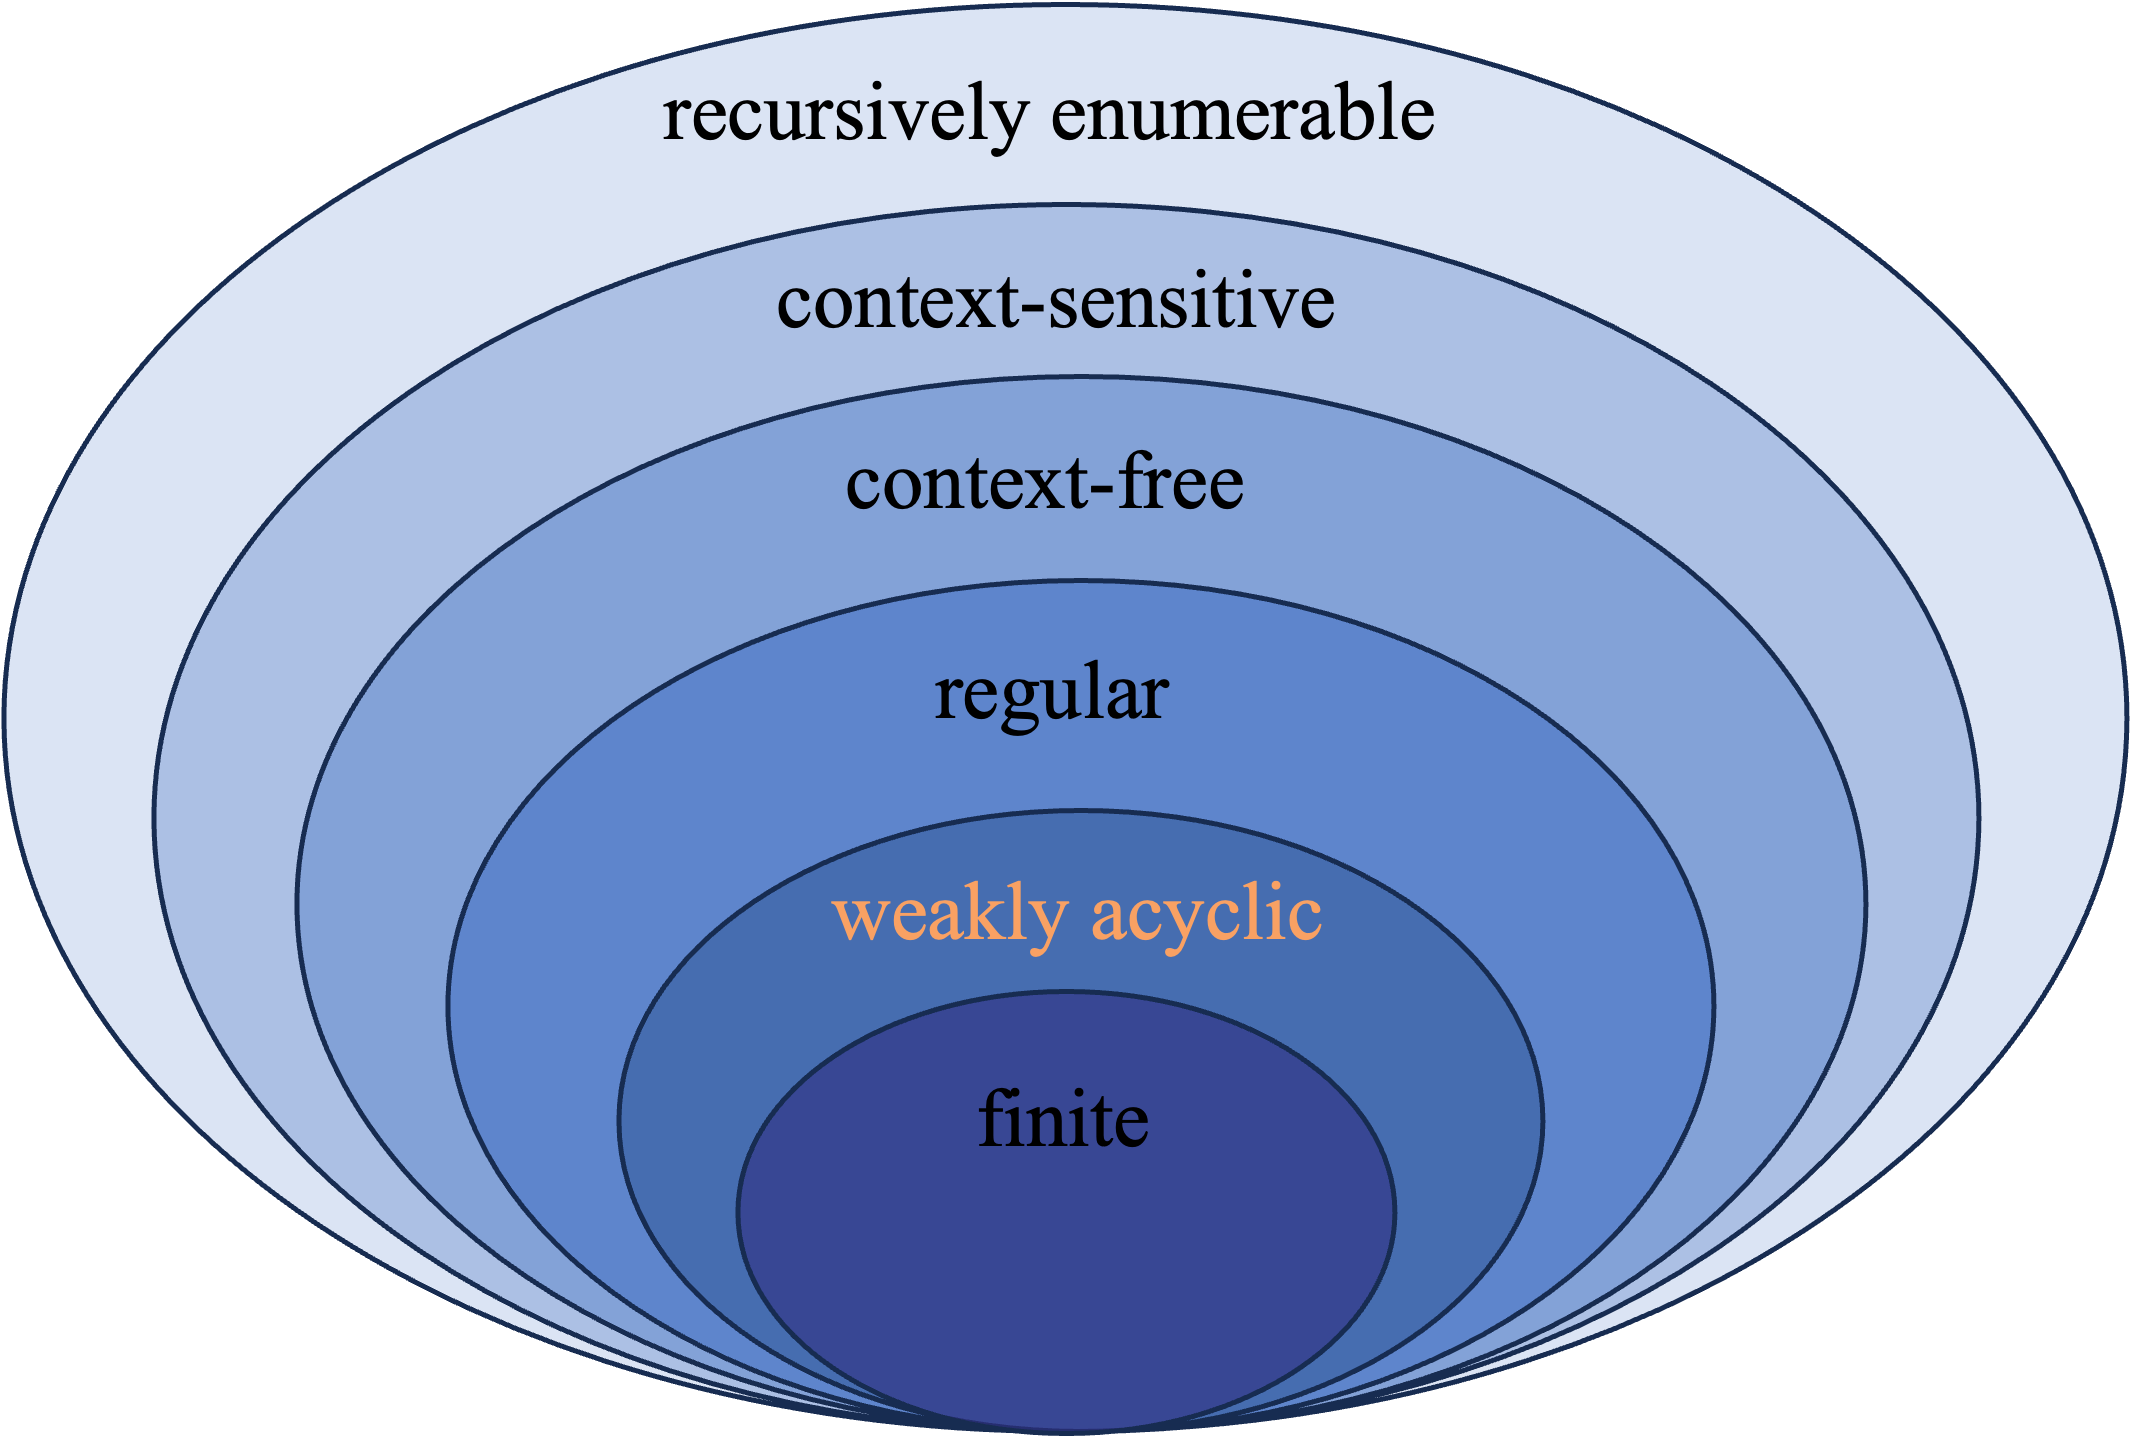
\includegraphics[scale=0.42]{./figures/languages.png}
\caption{Weakly Acyclic Classes in the Language Hierarchy}\label{fig:hierar}
\end{figure}


\subsection{Closure Properties}
Weakly acyclic languages are closed under union, intersection and complementation, but not under concatenation or Kleene star \cite{blondin_24}. 
\par 
As weakly acyclic languages can be described by DFAs, complementing a DFA still preserves its weakly acyclic structure. Furthermore, union is already present in the definition of weakly acyclic expressions in \autoref{sec:weakly_acyclic_regex}. Therefore, this class is also closed under intersection, which can be expressed with the combination of union and complementation. 
\par
Weakly acyclic languages are not closed under concatenation. The expressions $\bm{(a + b)^{*}}$ and $\bm{b}$ are weakly acyclic by themselves. The language of their concatenation $\bm{(a + b)^{*}b}$ is depicted in its unique minimal DFA in \autoref{fig:not-closed-concat}.

By Lemma~\autoref{lem:minimal} the minimal automaton of weakly acyclic language remains weakly acyclic. As this automaton contains a cycle of length 2, this language is not weakly acyclic. The same argumentation can be made for the Kleene star closure, with $\bm{ab}$ being a weakly acyclic language but $\bm{(ab)^{*}}$ represented in \autoref{fig:not-closed-kleene} is not weakly acyclic. 

\begin{figure}[H]
\centering 
	\begin{subfigure}{.30\textwidth}	
		\centering 
        \begin{tikzpicture}[>={Stealth[round]}]
    	\node[state, initial] (q1) {$q_{1}$};
    	\node[state, accepting, right of=q1] (q2) {$q_2$};
    	\draw   (q1) edge[loop above] node{$\bm{a}$} (q1)
            	(q1) edge[bend left, above] node{$\bm{b}$} (q2)
            	(q2) edge[loop above] node{$\bm{b}$} (q2)
            	(q2) edge[bend left, below] node{$\bm{a}$} (q1);
    	\end{tikzpicture}
    	\centering 
    	\caption{Minimal DFA of \\ $L(\bm{(a + b)^{*}b})$}\label{fig:not-closed-concat}
    \end{subfigure}
    \begin{subfigure}{.60\textwidth}
	\centering 
        \begin{tikzpicture}[>={Stealth[round]}]
    	\node[state, initial, accepting] (q1) {$q_1$};
    	\node[state, right of=q1] (q2) {$q_2$};
    	\node[state, right of=q2] (q3) {$q_3$};
    	\draw   (q1) edge[below] node{$\bm{a}$} (q2)
            	(q1) edge[bend right, below] node{$\bm{b}$} (q3)
            	(q2) edge[bend right, above] node{$\bm{b}$} (q1)
            	(q2) edge[below] node{$\bm{a}$} (q3)
            	(q3) edge[loop above] node{$\bm{a},\bm{b}$} (q3);
    	\end{tikzpicture}
    	\caption{Minimal DFA of $L(\bm{(ab)^{*}})$}\label{fig:not-closed-kleene}
    \end{subfigure}
     \caption{Not Weakly Acyclic DFAs}\label{fig:notwa}
\end{figure}
